\documentclass[compress]{beamer}
\usepackage{ifthen,verbatim}

\newcommand{\isnote}{}
\xdefinecolor{lightyellow}{rgb}{1.,1.,0.25}
\xdefinecolor{darkblue}{rgb}{0.1,0.1,0.7}

%% Uncomment this to get annotations
%% \def\notes{\addtocounter{page}{-1}
%%            \renewcommand{\isnote}{*}
%% 	   \beamertemplateshadingbackground{lightyellow}{white}
%%            \begin{frame}
%%            \frametitle{Notes for the previous page (page \insertpagenumber)}
%%            \itemize}
%% \def\endnotes{\enditemize
%% 	      \end{frame}
%%               \beamertemplateshadingbackground{white}{white}
%%               \renewcommand{\isnote}{}}

%% Uncomment this to not get annotations
\def\notes{\comment}
\def\endnotes{\endcomment}

\setbeamertemplate{navigation symbols}{}
\setbeamertemplate{headline}{\mbox{ } \hfill
\begin{minipage}{5.5 cm}
\vspace{-0.75 cm} \small
\end{minipage} \hfill
\begin{minipage}{4.5 cm}
\vspace{-0.75 cm} \small
\begin{flushright}
\ifthenelse{\equal{\insertpagenumber}{1}}{}{Jim Pivarski \hspace{0.2 cm} \insertpagenumber\isnote/\pageref{numpages}}
\end{flushright}
\end{minipage}\mbox{\hspace{0.2 cm}}\includegraphics[height=1 cm]{../cmslogo} \hspace{0.1 cm} \includegraphics[height=1 cm]{../tamulogo} \hspace{0.01 cm} \vspace{-1.05 cm}}

\begin{document}
\begin{frame}
\vfill
\begin{center}
\textcolor{darkblue}{\Large Update on global alignment of the muon system}

\vfill
\begin{columns}
\column{0.3\linewidth}
\begin{center}
\large
\textcolor{darkblue}{Jim Pivarski}
\end{center}
\end{columns}

\begin{columns}
\column{0.3\linewidth}
\begin{center}
\scriptsize
{\it Texas A\&M University}
\end{center}
\end{columns}

\vfill
11 May, 2009

\end{center}
\end{frame}

%% \begin{notes}
%% \item This is the annotated version of my talk.
%% \item If you want the version that I am presenting, download the one
%% labeled ``slides'' on Indico (or just ignore these yellow pages).
%% \item The annotated version is provided for extra detail and a written
%% record of comments that I intend to make orally.
%% \item Yellow notes refer to the content on the {\it previous} page.
%% \item All other slides are identical for the two versions.
%% \end{notes}

\small

%% \begin{frame}
%% \frametitle{Outline}
%% \begin{itemize}\setlength{\itemsep}{0.75 cm}
%% \item 
%% \end{itemize}
%% %% \hspace{-0.83 cm} \textcolor{darkblue}{\Large Outline2}
%% \end{frame}

%% \section*{First section}
%% \begin{frame}
%% \begin{center}
%% \Huge \textcolor{blue}{First section}
%% \end{center}
%% \end{frame}

\begin{frame}
\frametitle{Global alignment with tracks}
\begin{itemize}\setlength{\itemsep}{0.2 cm}
\item \textcolor{darkblue}{Status:} demonstrated high precision with collisions MC \mbox{and produced\hspace{-1 cm}} CRAFT barrel alignment with $20 < p_T < 100$~GeV tracks \mbox{(under review)\hspace{-1 cm}}
\item \textcolor{darkblue}{Goal:} move on to endcap alignment soon, where disk misalignments are known to be large
\item \textcolor{darkblue}{Meanwhile:} Jordan and Nhan performed their resolution diagnostics and provided very useful feedback
\begin{itemize}\setlength{\itemsep}{0.1 cm}
\item new DT alignment did not improve momentum-matching at all
\item what's the difference between alignment and diagnostics?  diagnostics have a higher $p_T$ cut
\item \textcolor{darkblue}{produced a muon alignment with $100 < p_T < 200$~GeV:}
\begin{enumerate}\setlength{\itemsep}{0.1 cm}
\item \textcolor{darkblue}{muon system seen to rotate 0.35~mrad}
\item \textcolor{darkblue}{big improvement in diagnostics plots (Jordan's talk)}
\end{enumerate}
\end{itemize}
\item \textcolor{darkblue}{This talk:} to determine what this means/find the underlying cause of the improvement
\end{itemize}
\end{frame}

\begin{frame}
\frametitle{The difference $p_T$ makes}

\vspace{0.3 cm}
\mbox{\hspace{-0.75 cm}}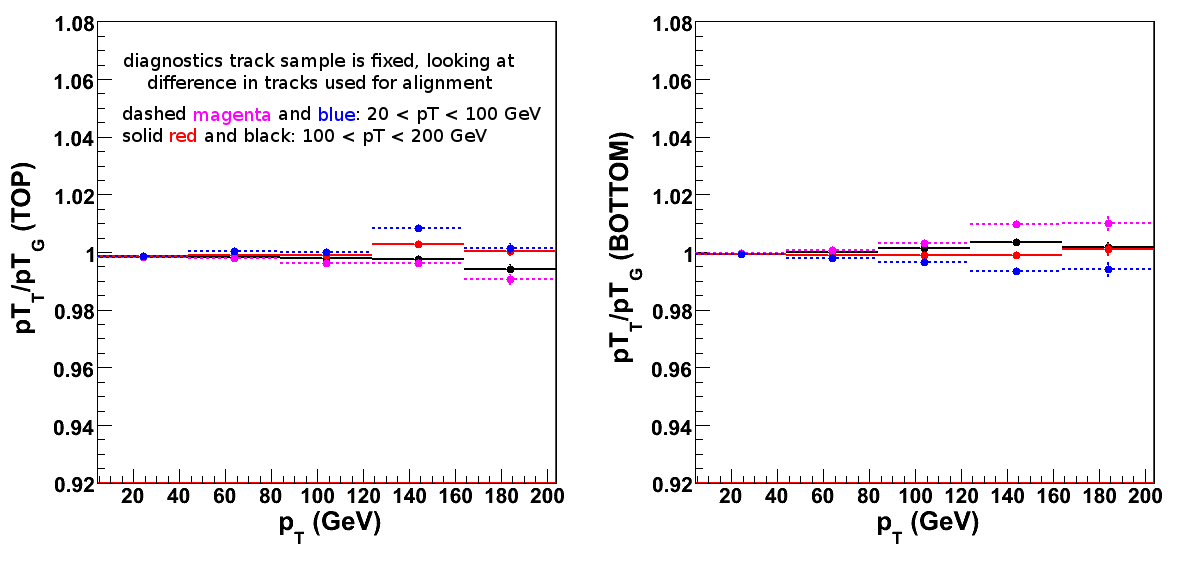
\includegraphics[width=1.15\linewidth]{plot_pTRatioVspT.png}

\vspace{-0.75 cm}
\mbox{ } \hfill \textcolor{darkblue}{\scriptsize Nhan Tran \hspace{-0.5 cm}}

\vspace{-0.15 cm}
\begin{itemize}
\item February and ``new'' $20 < p_T < 100$~GeV alignments lead to split track and tracker-muon discrepancy at high energies
\item Nhan tried adding 0.4~mrad rotation which empirically fixed things
\item \textcolor{darkblue}{Re-aligning using only $100 < p_T < 200$~GeV tracks yields a 0.35~mrad rotation and also improves resolution}
\end{itemize}
\end{frame}

\begin{frame}
\frametitle{How did the chambers move?}

\begin{itemize}
\item $\Delta \phi$ rotation around beamline (top row) and $r\phi$ position difference (bottom row) between high-$p_T$ and low-$p_T$, presented three ways
\item 0.35~mrad rotation, 0.04~mrad/m twist, and 3.2~mm spread
\end{itemize}

\mbox{\hspace{-0.75 cm}}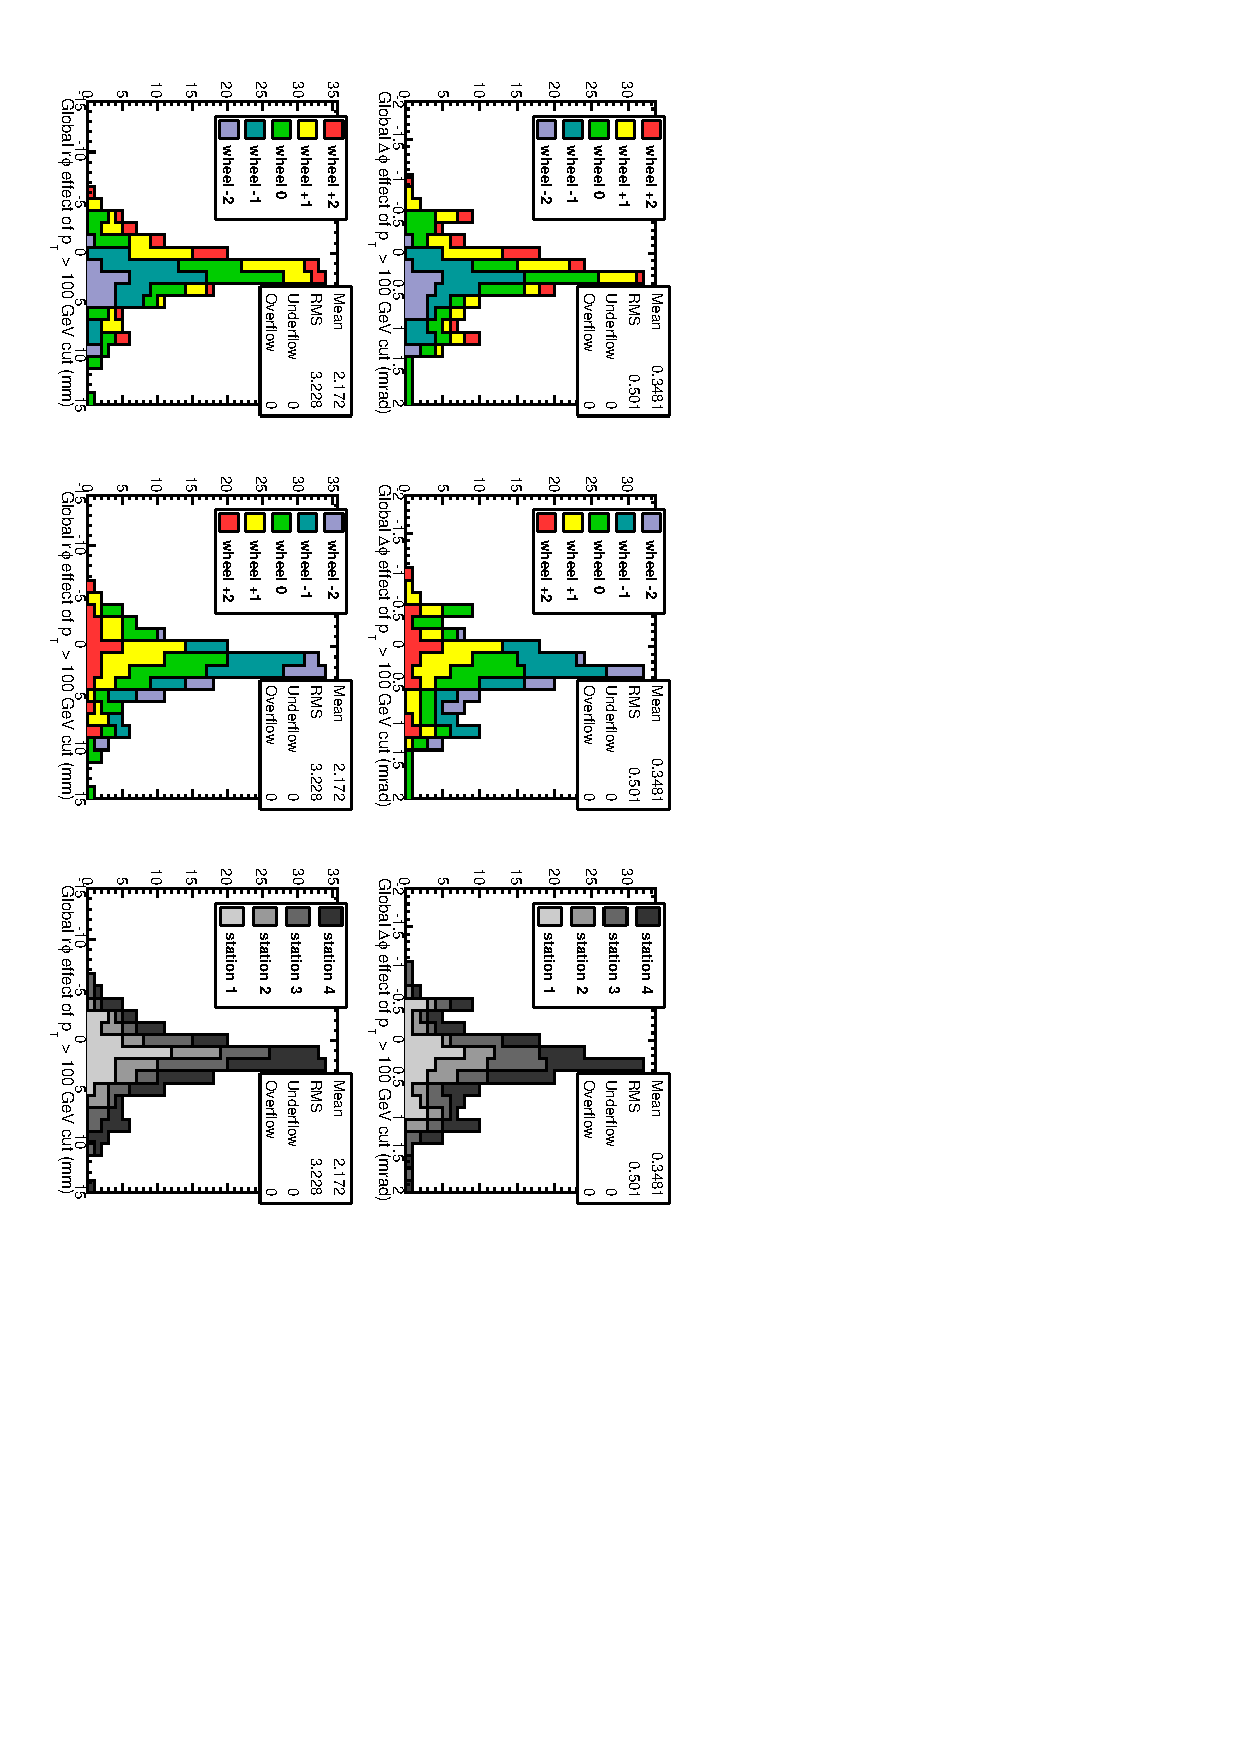
\includegraphics[height=1.15\linewidth, angle=90]{data_effect_of_100GeVcut3.pdf}
\end{frame}

\begin{frame}
\frametitle{\mbox{ }}

\begin{itemize}\setlength{\itemsep}{0.2 cm}
\item \textcolor{darkblue}{Fact:} Low-$p_T$ alignment is systematically rotated relative to high-$p_T$ alignment
\item \textcolor{darkblue}{Reminder:} each chamber is aligned to the tracker independently; chambers are {\it not} collectively aligned as a group
\begin{itemize}
\item nothing in the procedure correlates neighboring chambers with each other with higher precision than they are positioned in global coordinates
\end{itemize}
\item \textcolor{darkblue}{Mystery:} how could either alignment acquire a systematic offset?
\begin{itemize}\setlength{\itemsep}{0.2 cm}
\item \textcolor{darkblue}{Reminder:} all charge-antisymmetric effects like $\vec{B}(\vec{x})$ and $dE/dx$ are explicitly cancelled: must be charge-independent
\item \textcolor{darkblue}{Hypothesis \#1:} tracker ``curl'' weak mode projected onto muon system?  (tracker curl has tighter constraints than this)
\item \textcolor{darkblue}{Hypothesis \#2:} related to distribution of cosmic rays and ``sawtooth effect'' (open possibility, but it's complicated)
\end{itemize}
\end{itemize}
\end{frame}

\begin{frame}
\frametitle{Tracker curl hypothesis}
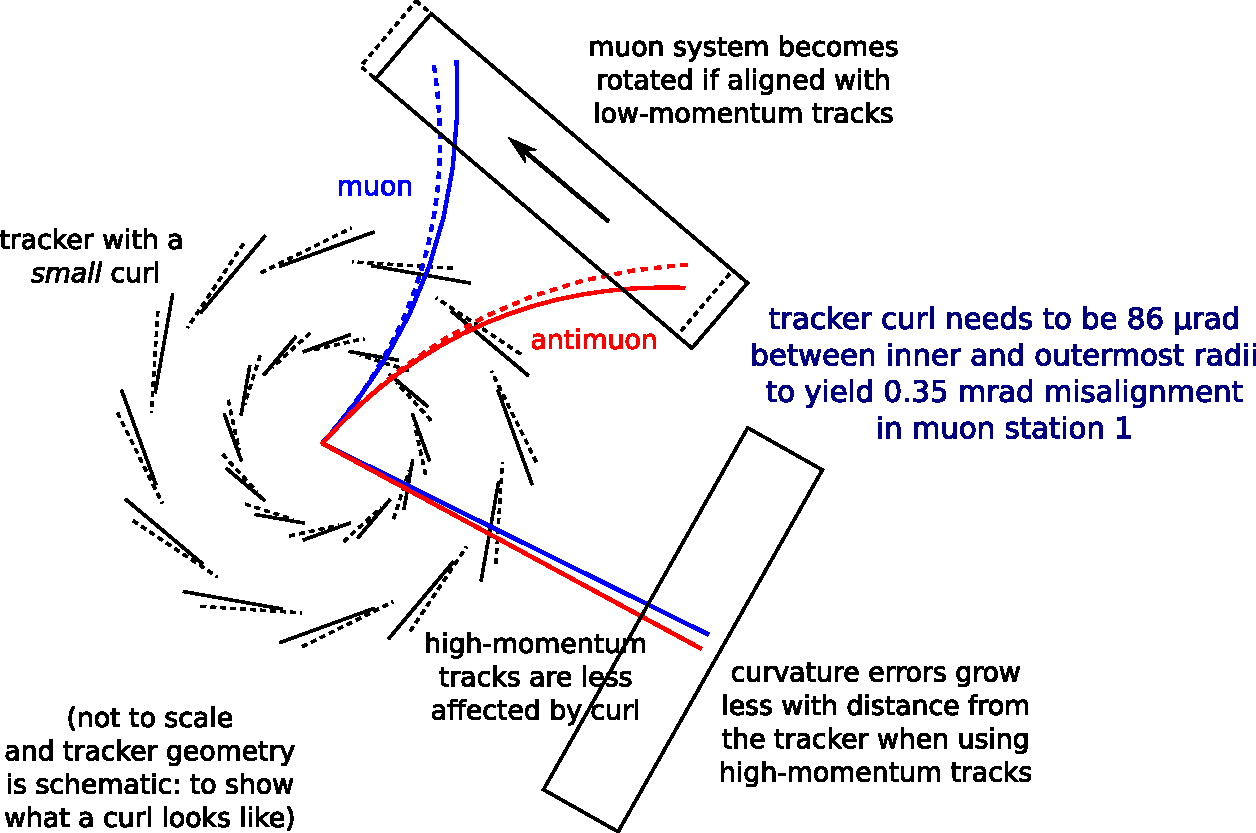
\includegraphics[width=\linewidth]{curl_explanation.pdf}
\end{frame}

\begin{frame}
\frametitle{Tracker curl constraints}

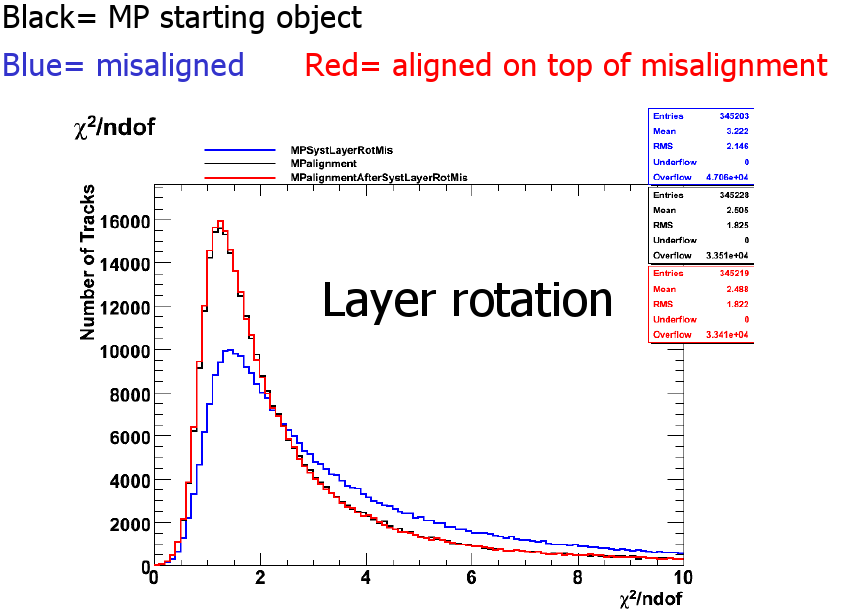
\includegraphics[width=0.55\linewidth]{tracks_are_sensitive_to_curl.png} \hfill 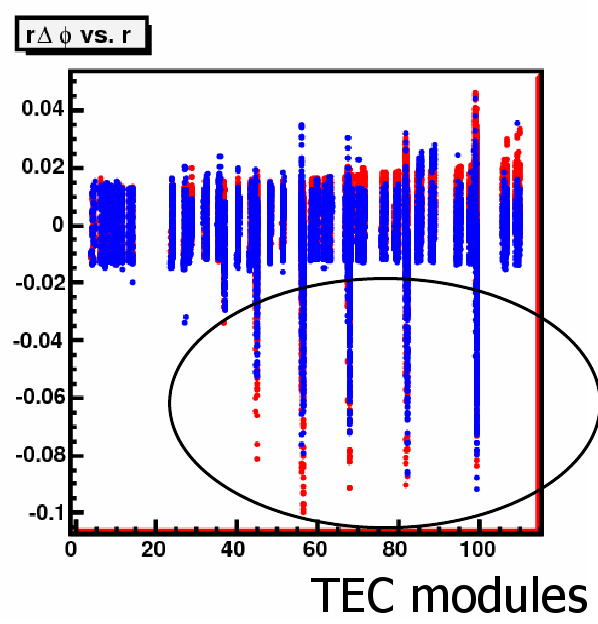
\includegraphics[width=0.35\linewidth]{curl_is_not_86microns.png}

\begin{itemize}
\item Studies performed in CRAFT data \hfill \textcolor{darkblue}{\scriptsize Zijin Guo, Roberto Castello}
\item \textcolor{darkblue}{Left:} tracker tracks are sensitive to 300~$\mu$rad curl (\textcolor{blue}{blue:\ adding curl worsens $\chi^2$} and \textcolor{red}{red:\ re-aligning restores it})
\item \textcolor{darkblue}{Right:} also restores wafer positions within 150~$\mu$rad \mbox{except TEC\hspace{-1 cm}}
\begin{itemize}
\item TEC not used in muon alignment; not relevant here
\item restored chamber positions randomly distributed around zero: \textcolor{darkblue}{no {\it systematic} trend on the scale of 86~$\mu$rad}
\end{itemize}
\end{itemize}
\end{frame}

\begin{frame}
\frametitle{Tracker curl conclusion}

\vspace{-1 cm}
\begin{itemize}
\item Tracker curl hypothesis requires a larger systematic trend than dedicated systematics studies allow
\item {\it Might} account for the spread, but not the systematic rotation
\end{itemize}

\vfill
\hspace{-0.83 cm} \textcolor{darkblue}{\Large Muon residuals studies: outline}

\vspace{0.4 cm}
\begin{enumerate}
\item \textcolor{darkblue}{Reminder:} ``sawtooth effect'' in DTs still unexplained
\item We see low-$p_T$/high-$p_T$ rotation in raw residuals
\item Sawtooth effect is related to $p_T$ effect, but not in a simple way
\end{enumerate}
\end{frame}

\begin{frame}
\frametitle{Sawtooth effect}

\vspace{0.25 cm}
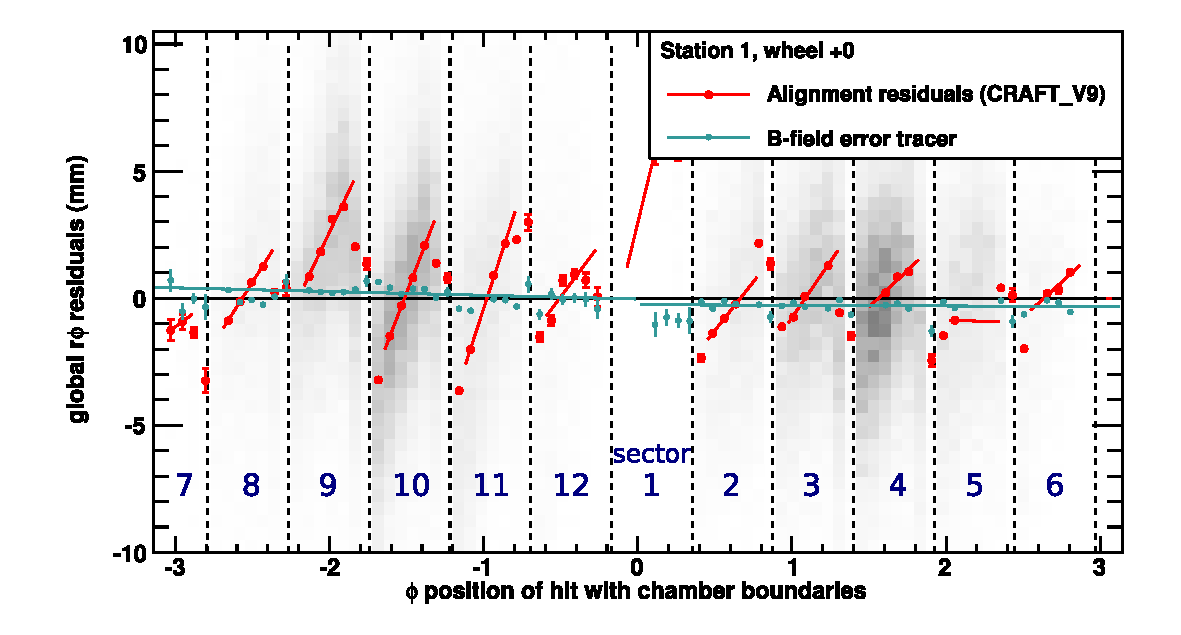
\includegraphics[width=\linewidth]{DTrphiVsPhi_st1_whC.pdf}

\vspace{-0.25 cm}
\hfill {\scriptsize old plot, shown in Torino}

\begin{itemize}
\item Global $r\phi$ ($\Delta x$) residual vs.\ $\phi$ trends, unrelated to \mbox{rigid-body alignment\hspace{-1 cm}}
\begin{itemize}\setlength{\itemsep}{0.1 cm}
\item $\phi$ is equivalent to local $x$ position and $\frac{dx}{dz}$ \mbox{entrance angle\hspace{-1 cm}}
\item $\Delta x$ residuals correlated with $\Delta \frac{dx}{dz}$ angular residuals \mbox{(understood)\hspace{-1 cm}}
\end{itemize}
\end{itemize}
\end{frame}

\begin{frame}
\frametitle{Sawtooth in one chamber}

\vspace{0.35 cm}
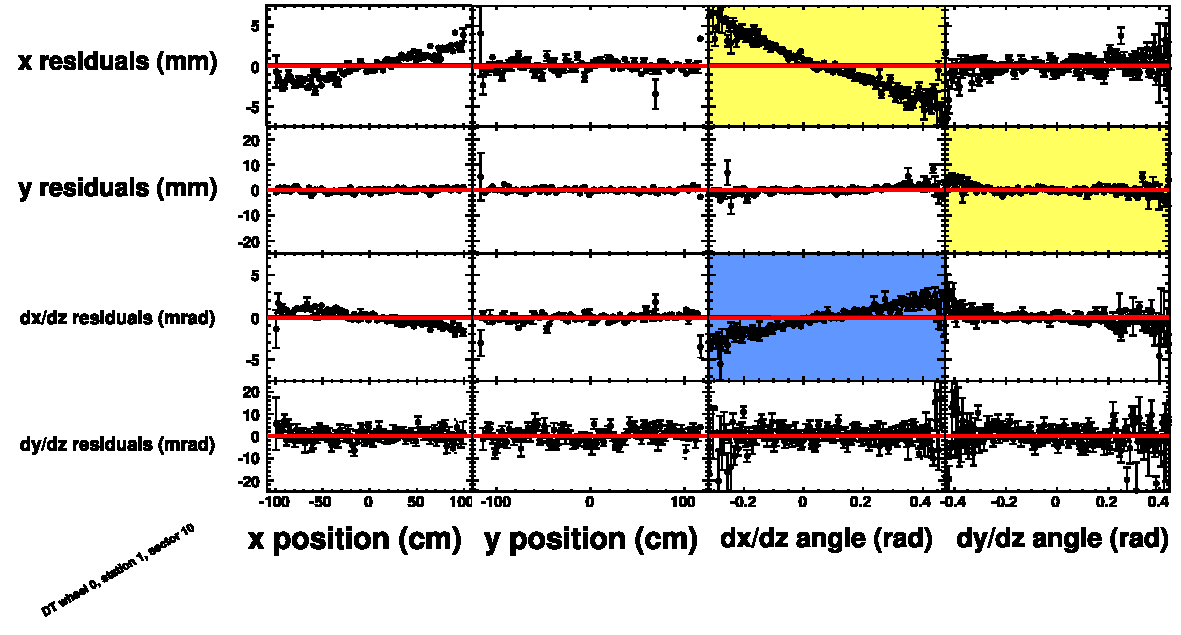
\includegraphics[width=\linewidth]{datafit_wh0st1sec10_highp.pdf}

\vspace{-0.35 cm}
\begin{itemize}
\item These are all of the constraints on a single chamber alignment fit
\begin{itemize}\setlength{\itemsep}{0.1 cm}
\item sawtooth seen in correlated $x$ and $\frac{dx}{dz}$, but more strongly \mbox{in latter\hspace{-1 cm}}
\item yellow boxes: {\it both} must be sloped for radial ($z$) misalignment
\item blue/grey box: must be $(1 + (\frac{dx}{dz})^2)$ for $\phi_y$ angle misalignment
\item 6-DOF alignment cannot eliminate sawtooth trend
\end{itemize}
\end{itemize}
\end{frame}

\begin{frame}
\frametitle{Sawtooth distribution: low-$p_T$}

\begin{itemize}
\item Distribution of the effect (from separate linear fits to $\Delta \frac{dx}{dz}$ vs.\ $\frac{dx}{dz}$)
\begin{itemize}
\item mostly depends on station number (largest in station~1)
\end{itemize}
\end{itemize}

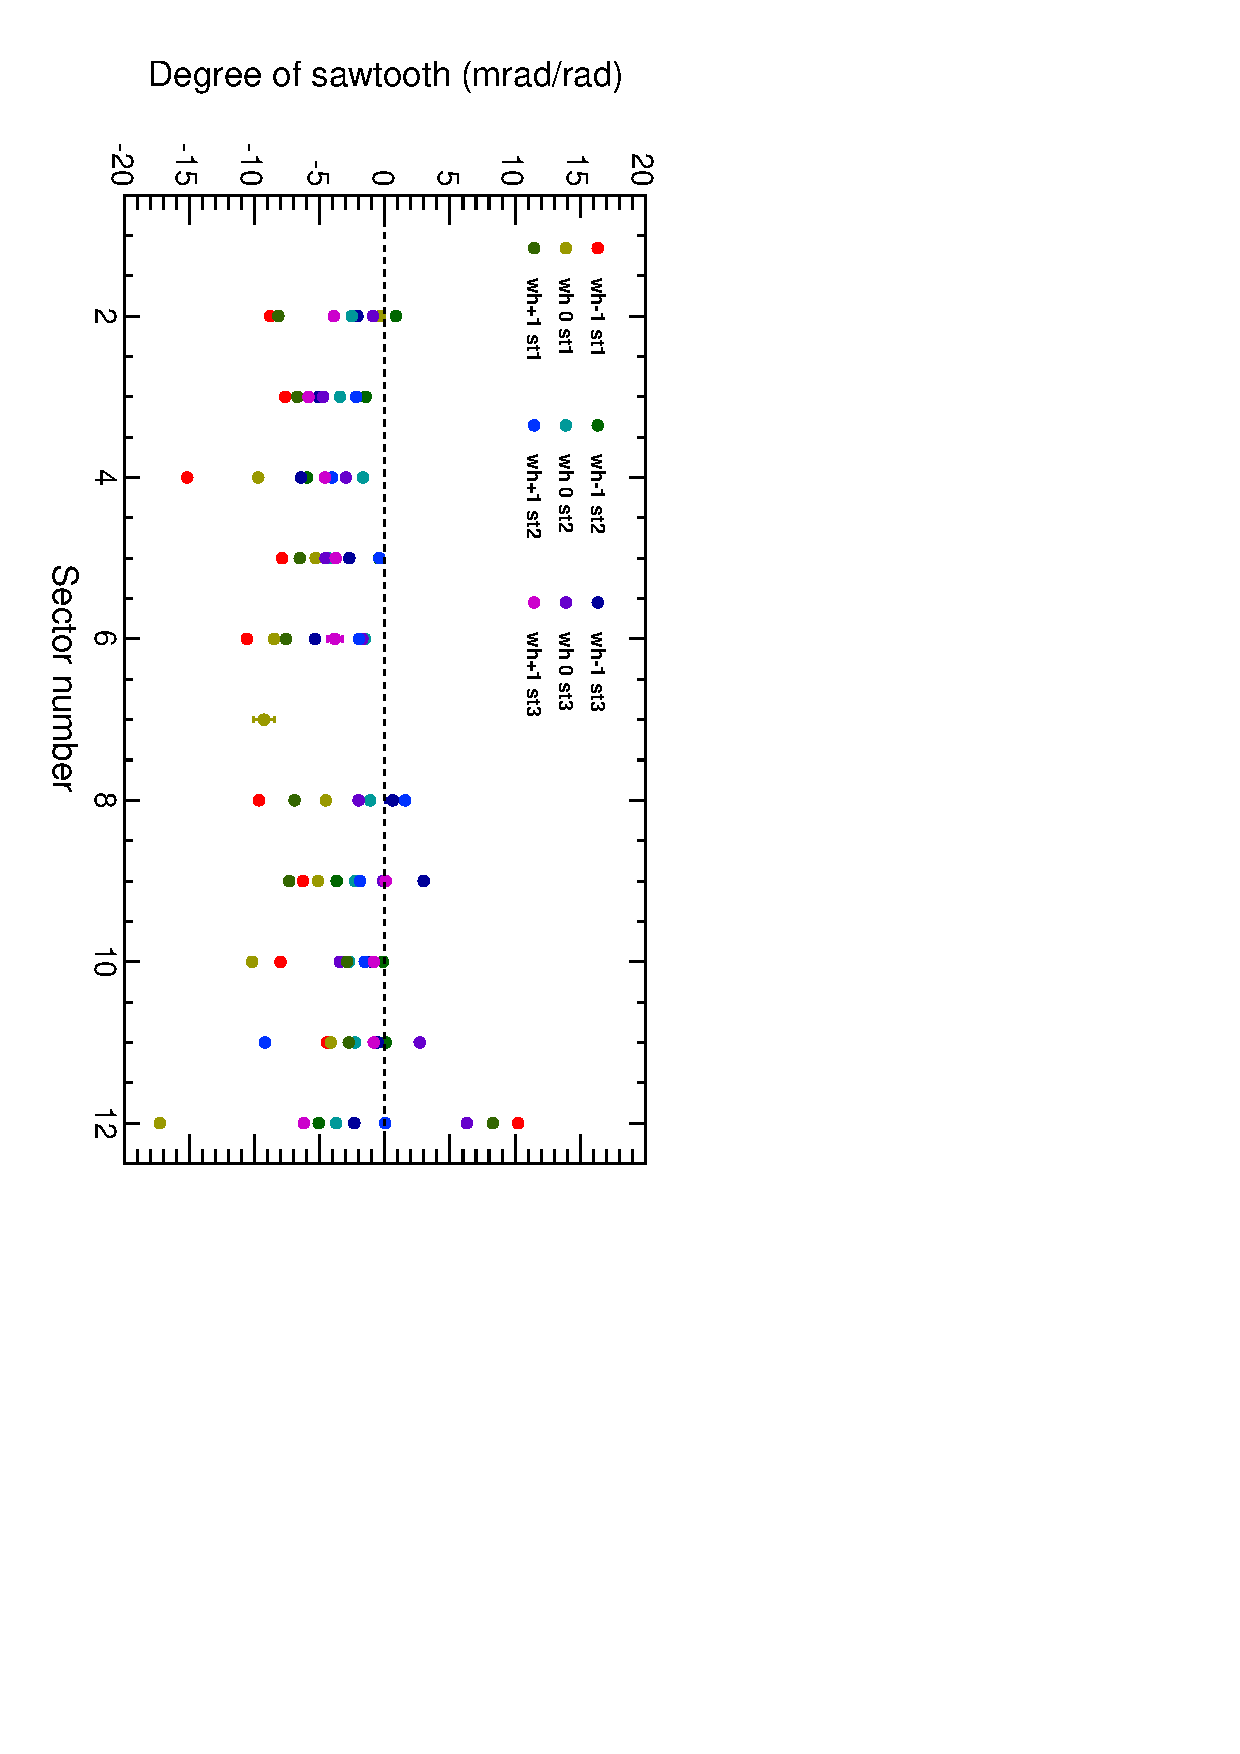
\includegraphics[height=\linewidth, angle=90]{sawtooth_bysector_lowp.pdf}
\end{frame}

\begin{frame}
\frametitle{Sawtooth distribution: high-$p_T$}

\begin{itemize}
\item Same thing with $100 < p_T < 200$~GeV tracks
\begin{itemize}\setlength{\itemsep}{0.1 cm}
\item distribution more centered
\item $2 + 4\sin\phi$ curve is vaguely suggested\ldots\ a clue?
\end{itemize}
\end{itemize}

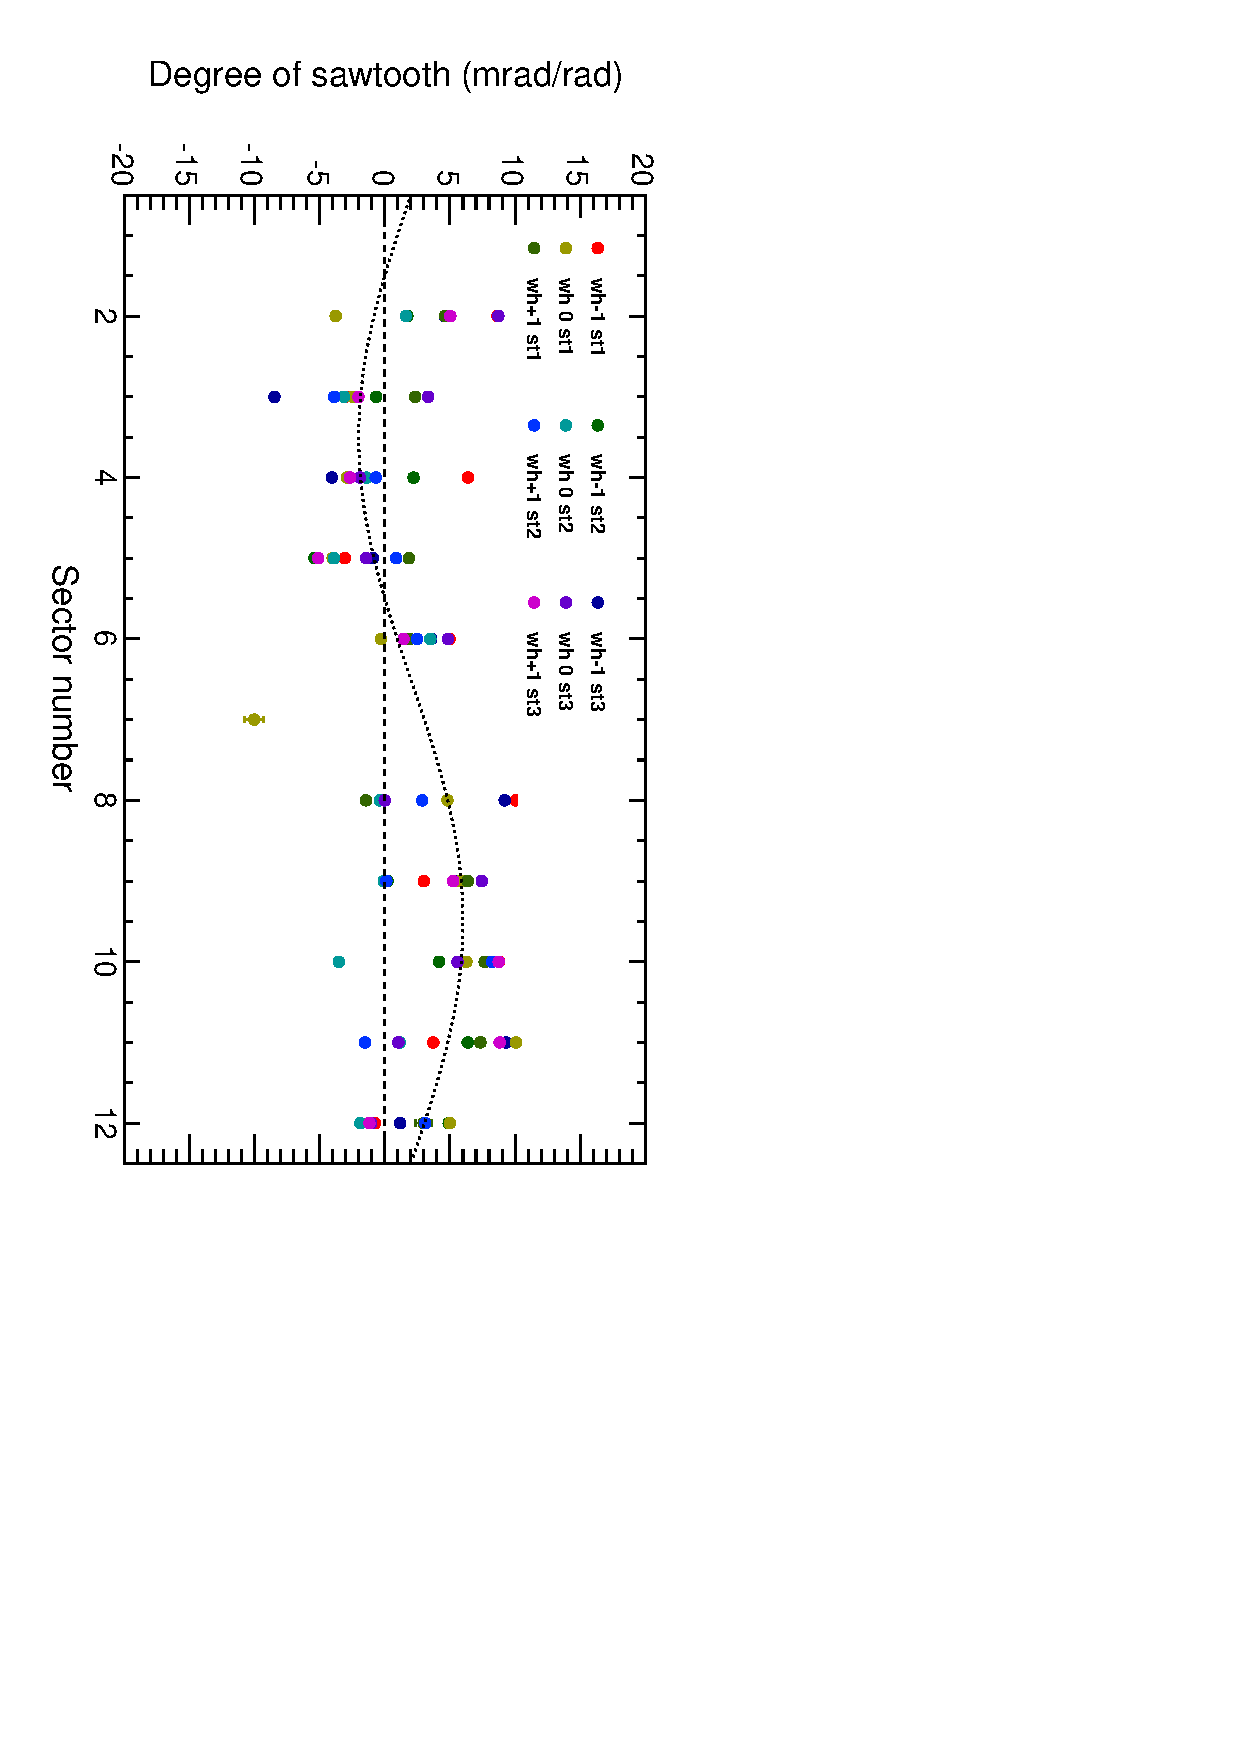
\includegraphics[height=\linewidth, angle=90]{sawtooth_bysector_highp.pdf}
\end{frame}

\begin{frame}
\frametitle{$p_T$ effect in raw residuals}

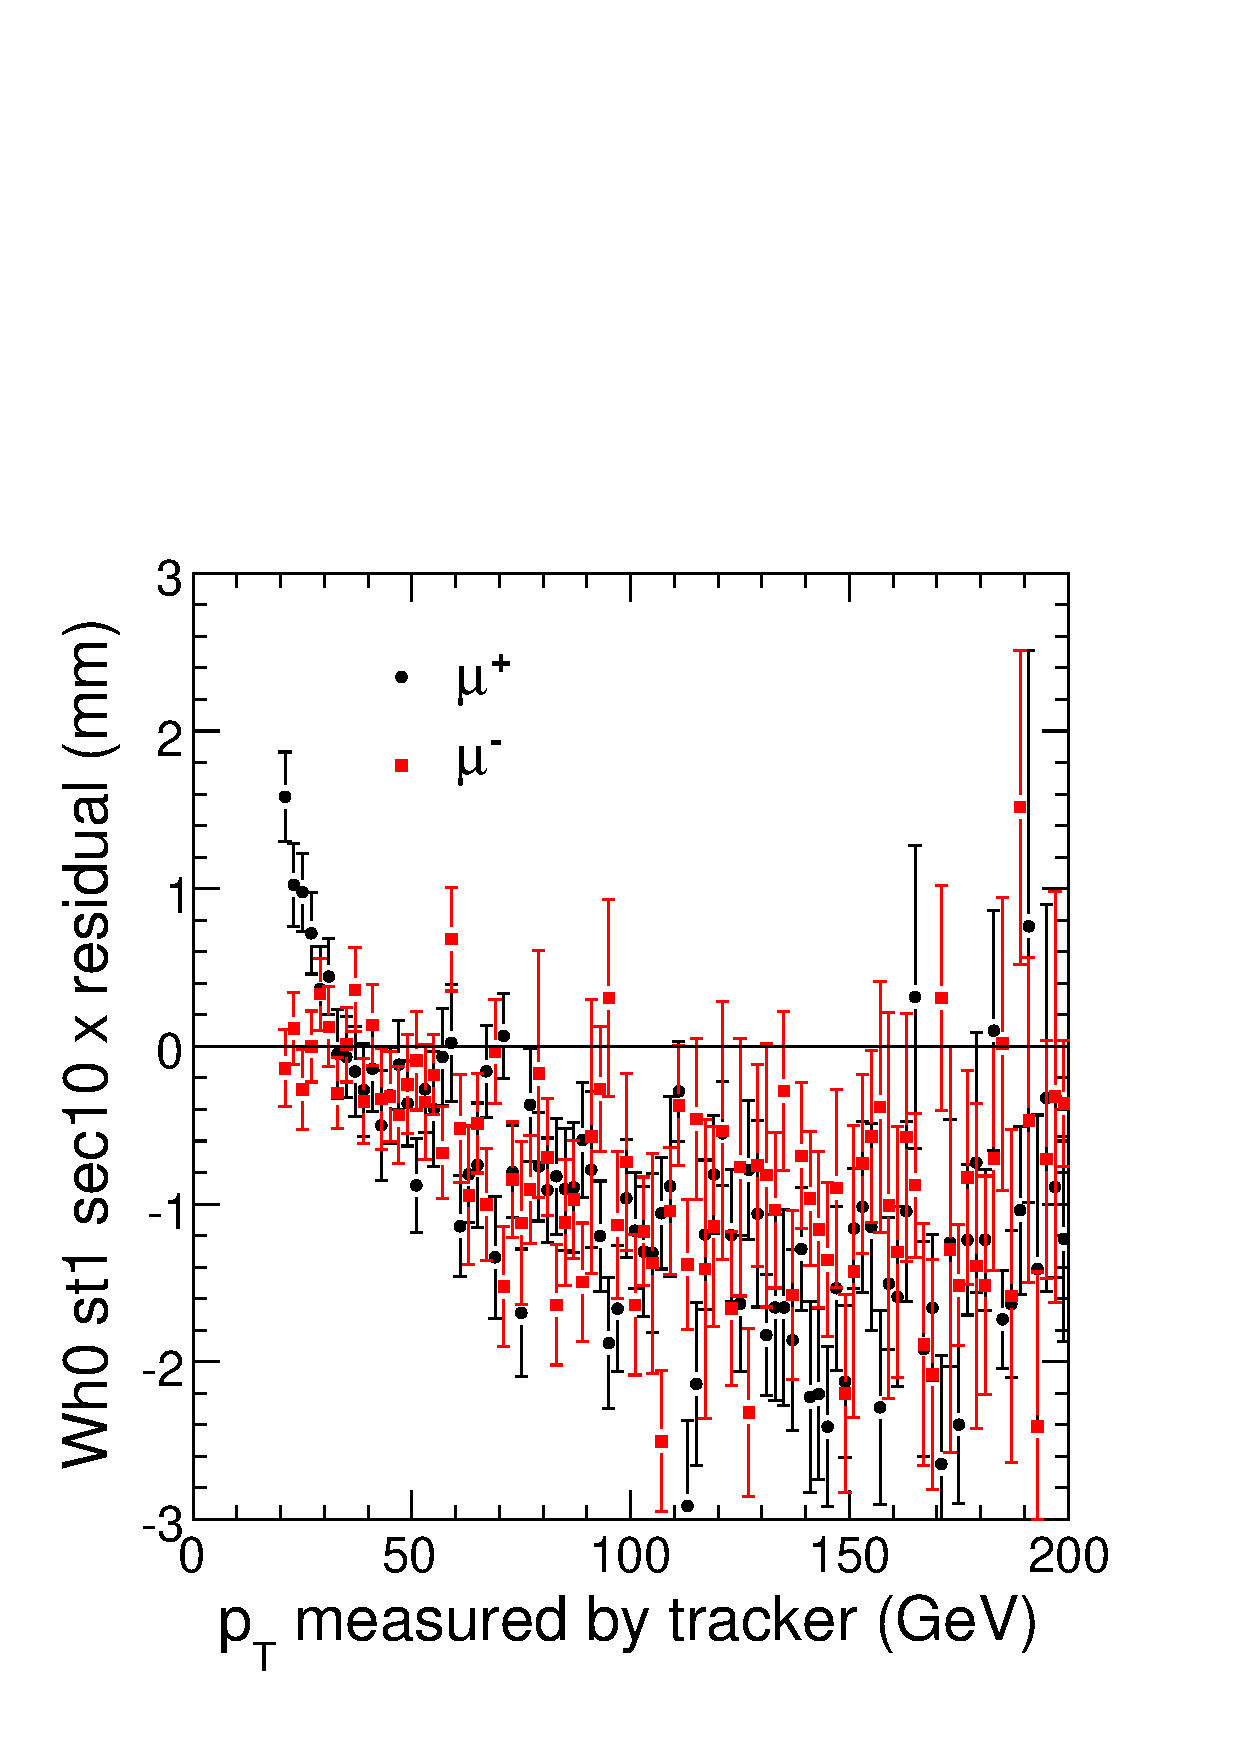
\includegraphics[width=0.45\linewidth]{resid_vs_pt.pdf} \hfill 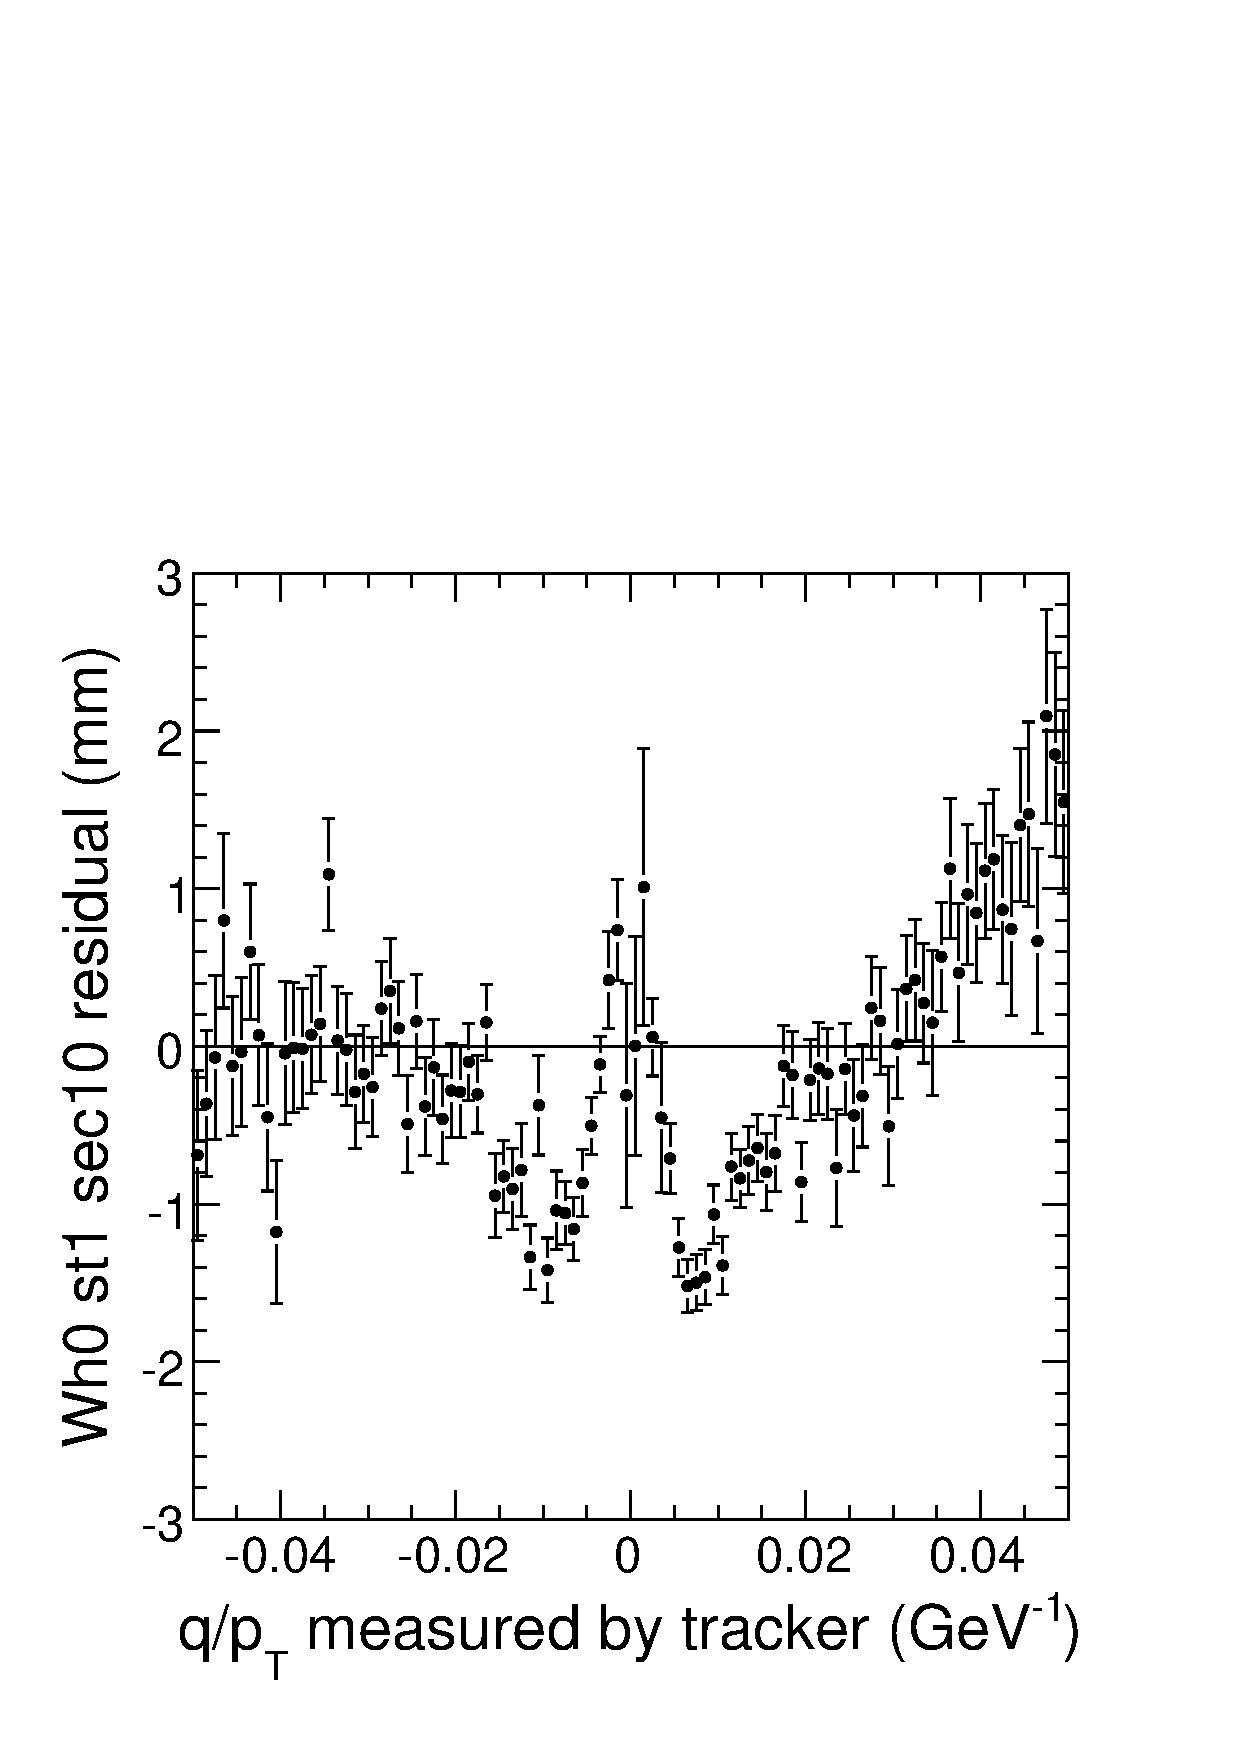
\includegraphics[width=0.45\linewidth]{resid_vs_qoverpt.pdf}

\begin{itemize}
\item Same chamber as page 10 {\scriptsize (wheel~0, station~1, sector~10, bottom of barrel)}
\item $\mu^+$/$\mu^-$ splitting at low-$p_T$ can be due to $\vec{B}(\vec{x})$ or $dE/dx$ errors
\item Drifts to lower residual at high-$p_T$, independent of charge
\begin{itemize}\setlength{\itemsep}{0.1 cm}
\item high-$p_T$ alignment: $100 < p_T < 200$~GeV
\item returns at very high-$p_T$???  not seen in all chambers\ldots
\end{itemize}
\end{itemize}
\end{frame}

\begin{frame}
\frametitle{$\frac{dx}{dz}$ (sawtooth variable) and $p_T$}

\begin{columns}
\column{0.35\linewidth}
\vspace{0.25 cm}
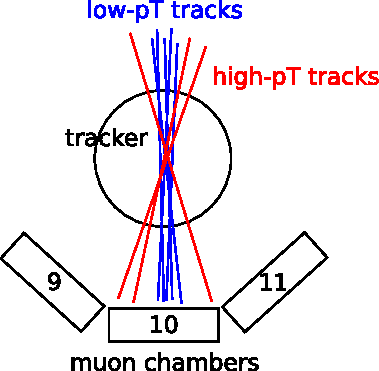
\includegraphics[width=\linewidth]{cosmics_are_nasty.pdf}

\column{0.65\linewidth}
\begin{itemize}
\item Still looking at only one chamber, note that $\frac{dx}{dz}$ and $p_T$ are related
\item Expected because low-$p_T$ muons are more vertically collimated by the Earth
\item Unique to cosmic rays: in $\phi$-symmetric collisions, $p_T$ and $\frac{dx}{dz}$ will be independent
\end{itemize}
\end{columns}

\vspace{-0.25 cm}
\begin{columns}
\column{0.2\linewidth}
\begin{itemize}
\item Low-$p_T$ band is sloped because of $\vec{B}$
\end{itemize}

\column{0.8\linewidth}
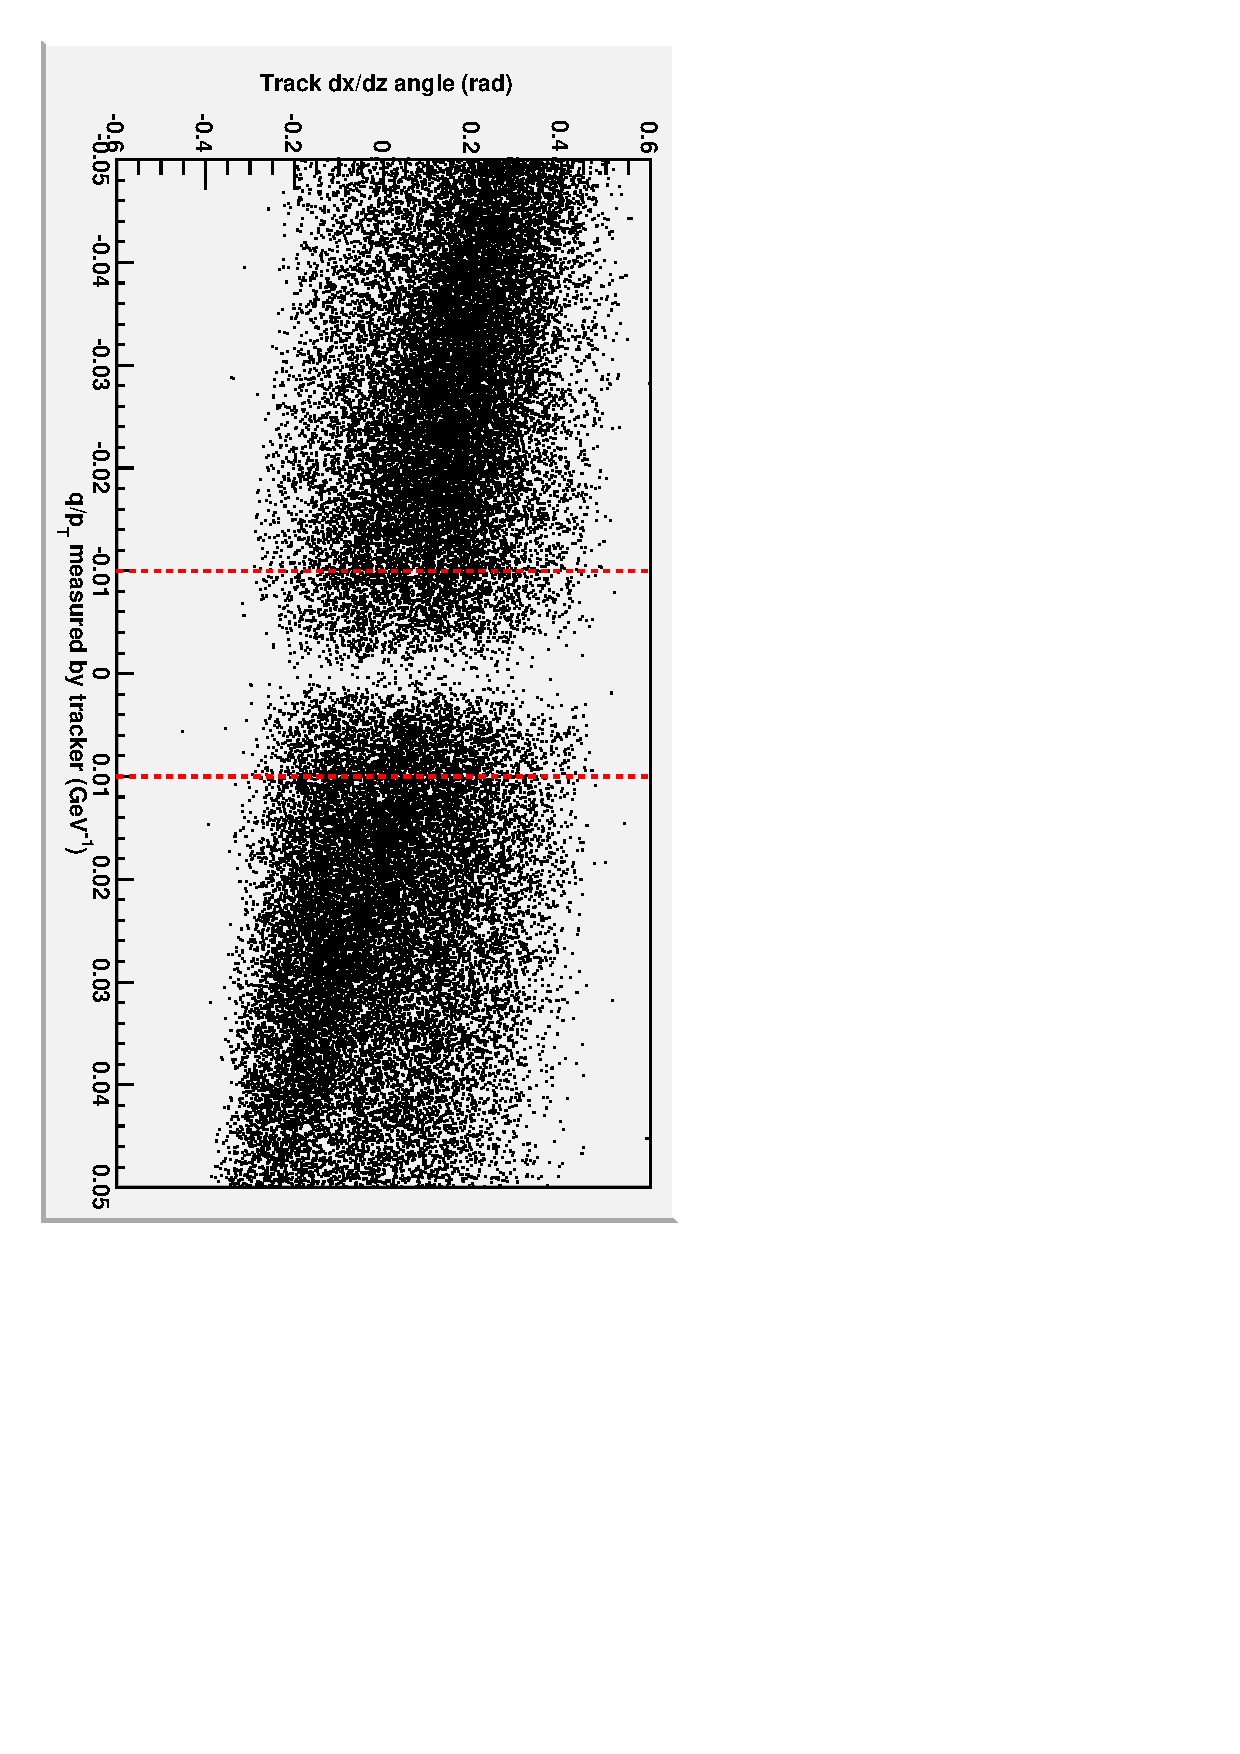
\includegraphics[height=\linewidth, angle=90]{sawtooth_and_qoverpt2.pdf}
\end{columns}
\end{frame}

\begin{frame}
\frametitle{Is it just integration?}

\begin{itemize}
\item Muons in different $q/p_T$ slices are sensitive to different parts of the sawtooth line
\item But if this were the only effect, \textcolor{red}{$-0.05 < q/p_T
  < -0.04$~GeV$^{-1}$} and \textcolor{violet}{$0.04 < q/p_T <
  0.05$~GeV$^{-1}$} would have opposite-signed residuals
\item \textcolor{darkblue}{They don't: we saw that the $p_T$ effect is charge-independent}
\end{itemize}

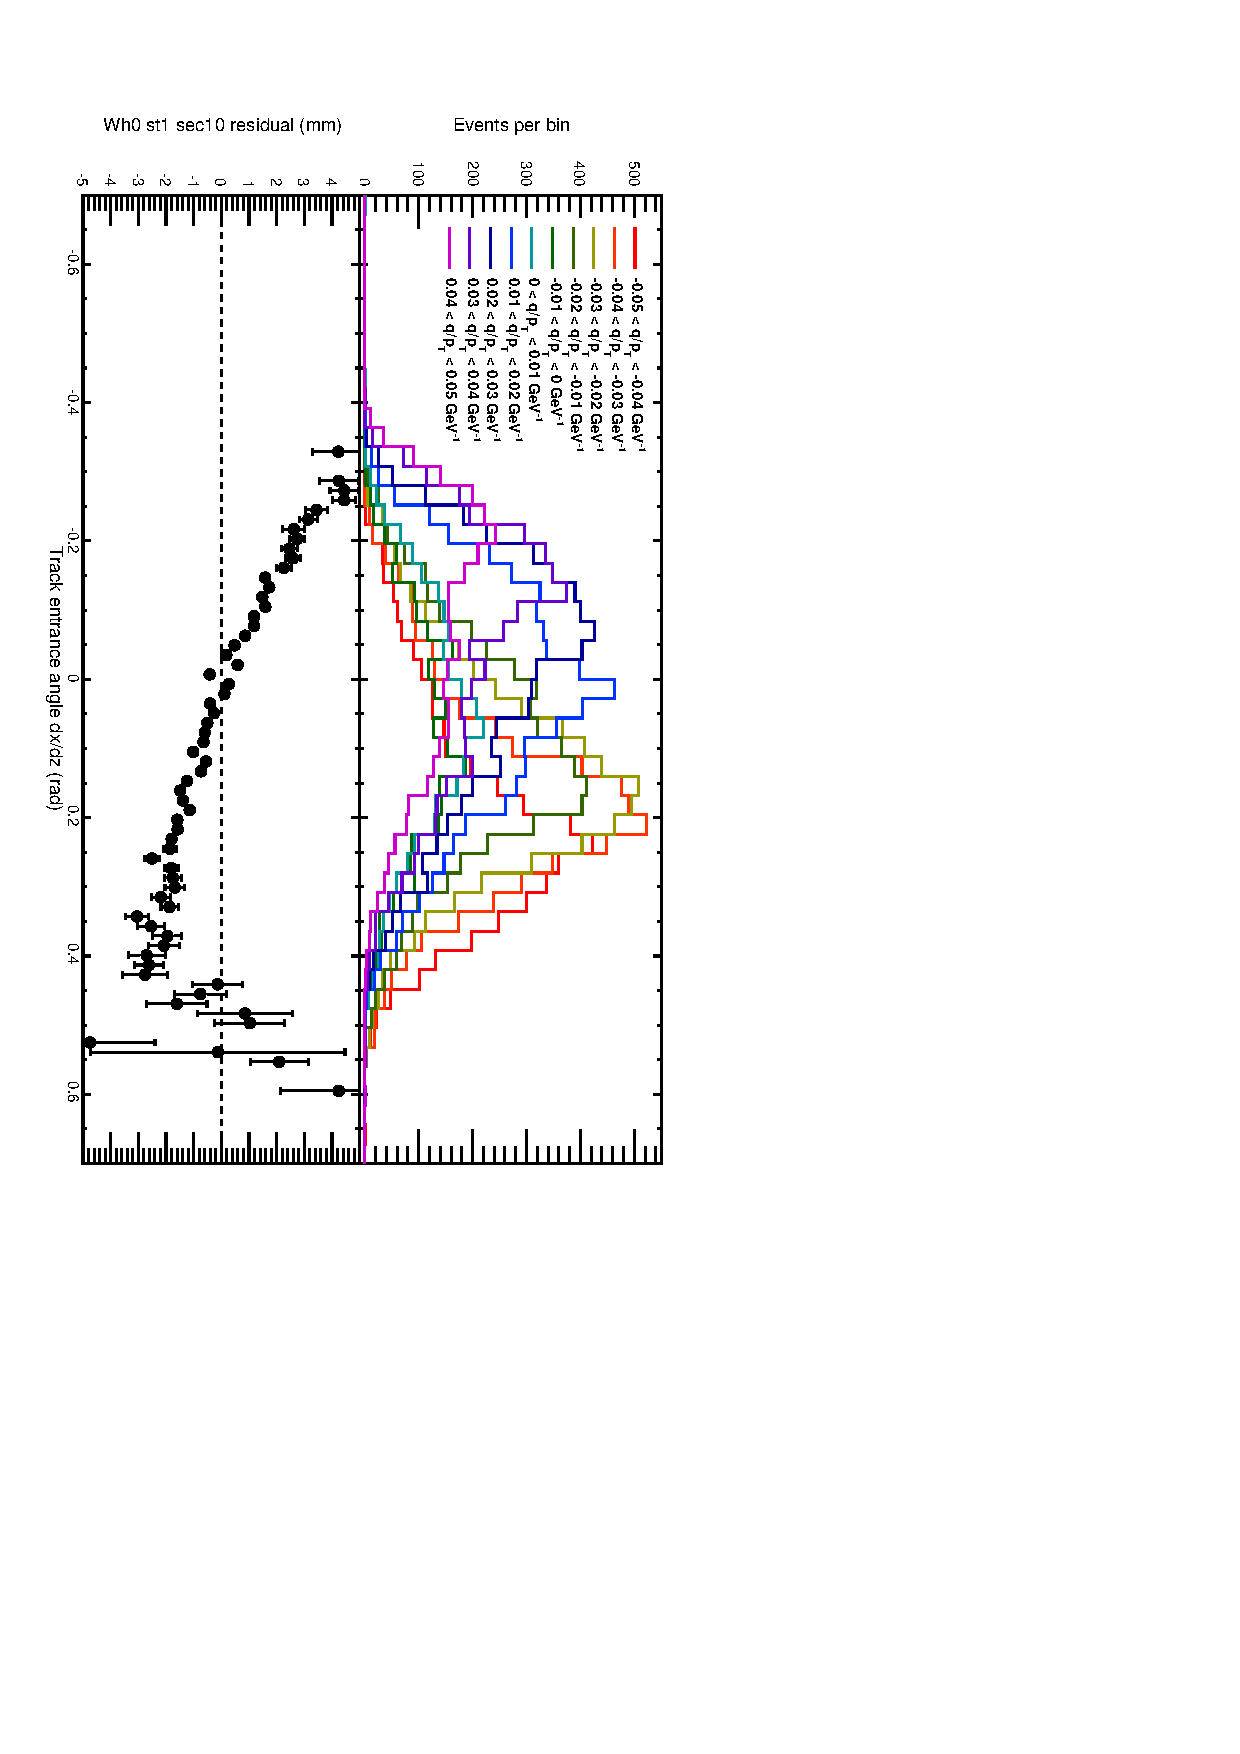
\includegraphics[height=\linewidth, angle=90]{sawtooth_and_qoverpt.pdf}
\end{frame}

\begin{frame}
\frametitle{Dependence on both $p_T$ and $\frac{dx}{dz}$}

\begin{itemize}
\item Residuals (greyscale, mm) are a function of both $p_T$ and $\frac{dx}{dz}$
\begin{itemize}\setlength{\itemsep}{0.1 cm}
\item sawtooth effect is vertical trend from dark to light
\item $p_T$ effect is horizontal darkening in center
\item still one chamber only: different for each chamber, \mbox{due to geometry\hspace{-1 cm}}
\end{itemize}

\end{itemize}

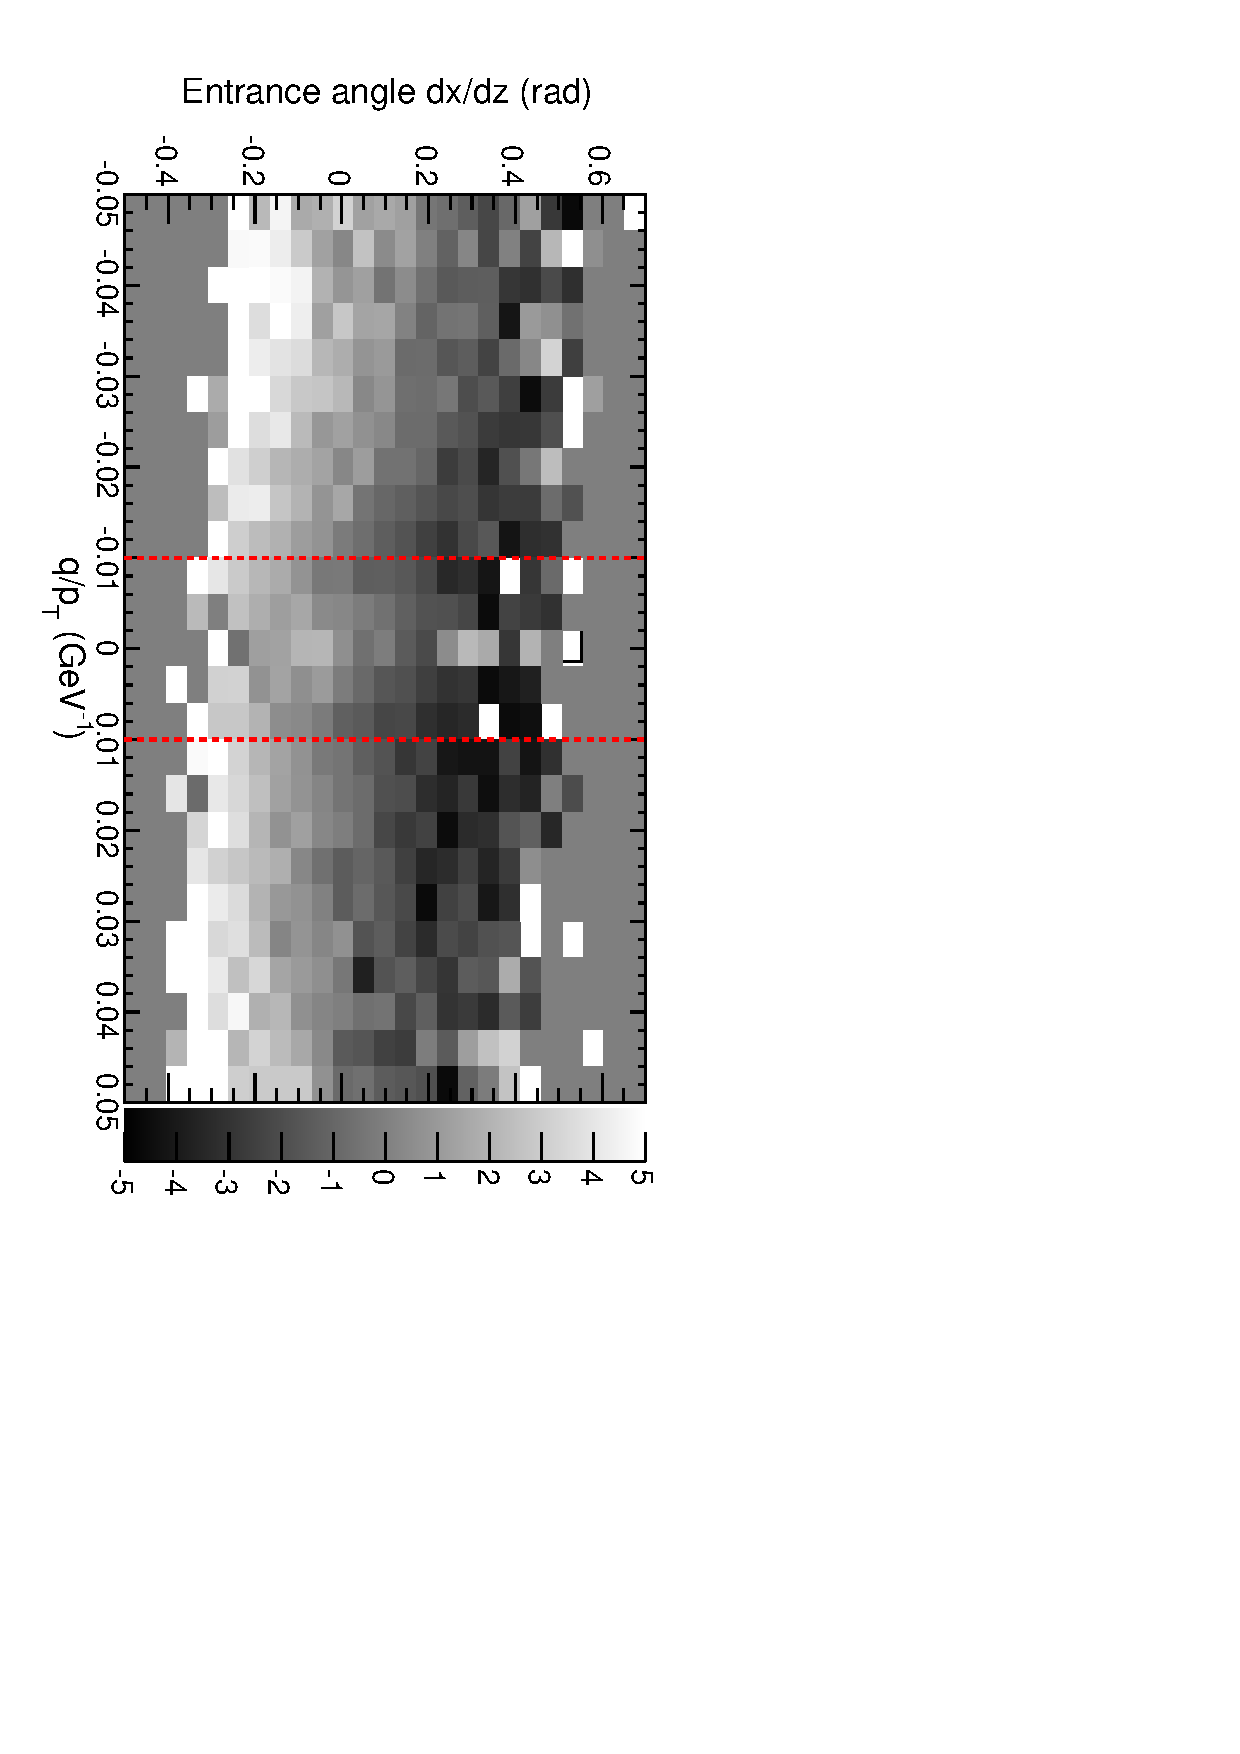
\includegraphics[height=\linewidth, angle=90]{sawtooth_qoverpt_complicated2.pdf}
\end{frame}

\begin{frame}
\frametitle{Conclusions}

\begin{itemize}\setlength{\itemsep}{0.2 cm}
\item \textcolor{darkblue}{Alignment performed with $100 < p_T < 200$~GeV cut clearly improves resolution (see Jordan's talk)}
\begin{itemize}
\item \textcolor{darkblue}{for the first time, tracker $+$ muon outperforms tracker alone at high $p_T$}
\end{itemize}

\item High-$p_T$ alignment results in a systematic 0.35~mrad rotation, consistent with Nhan's empirical study

\item A $p_T$-dependent rotation could be caused by tracker curl
\begin{itemize}\setlength{\itemsep}{0.1 cm}
\item we would need 86~$\mu$rad in the tracker to explain 0.35~mrad in the muon system
\item \textcolor{darkblue}{tracker studies rule out systematic trends on this scale}
\item {\it might} account for the spread
\end{itemize}

\item Sawtooth effect is still unexplained (volunteers appreciated!)

\item Sawtooth and $p_T$ effects intermingle because cosmic ray
  distribution is a function of both entrance angle and $p_T$

\item One effect is not derived from the other simply by integration
\end{itemize}

\label{numpages}
\end{frame}

\end{document}
